\hypertarget{fungi}{%
\chapter{Fungi}\label{fungi}}

Fungi (singular: fungus) are heterotrophic uni- or multicellular eukaryotic organisms with external digestion and include microorganisms such as yeasts and molds, as well as the more familiar mushrooms. These organisms are classified as a kingdom, which is separate from the other eukaryotic life kingdoms of plants and animals.



\begin{figure}

{\centering 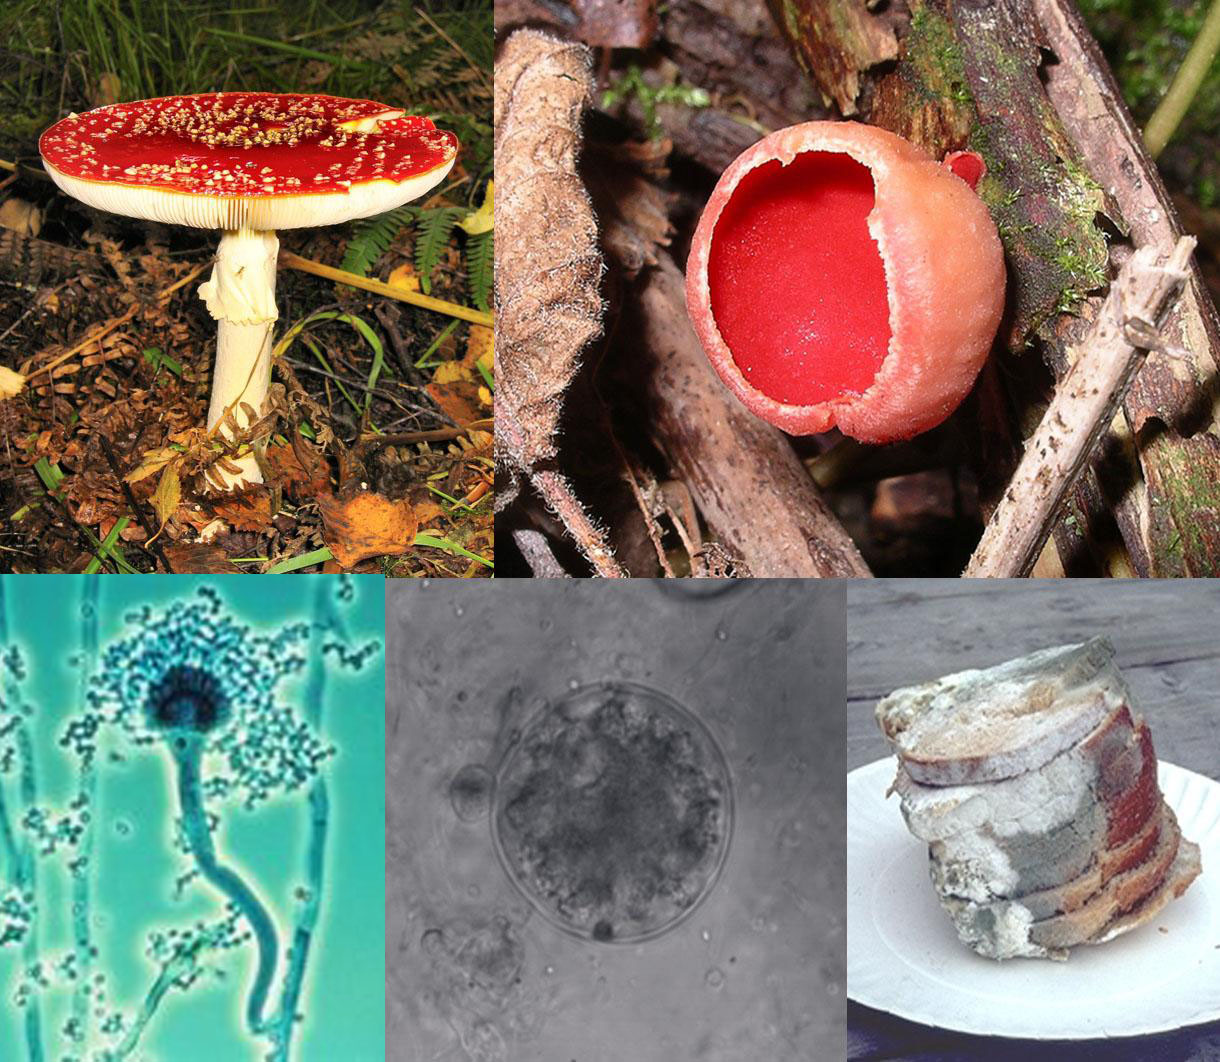
\includegraphics[width=0.7\linewidth]{./figures/fungi/Fungi_collage} 

}

\caption{\href{https://commons.wikimedia.org/wiki/File:Fungi_collage.jpg}{A collage of five fungi (clockwise from top-left):} a mushroom with a flat, red top with white-spots, and a white stem growing on the ground; a red cup-shaped fungus growing on wood; a stack of green and white moldy bread slices on a plate; a microscopic, spherical grey semitransparent cell, with a smaller spherical cell beside it; a microscopic view of an elongated cellular structure shaped like a microphone, attached to the larger end is a number of smaller roughly circular elements that collectively form a mass around sites.}\label{fig:fungidiversity}
\end{figure}

A characteristic that places fungi in a different kingdom from plants, bacteria, and some protists is chitin in their cell walls. Similar to animals, fungi are heterotrophs; they acquire their food by absorbing dissolved molecules, typically by secreting digestive enzymes into their environment. Fungi do not photosynthesize. Growth is their means of mobility, except for spores (a few of which are flagellated), which may travel through the air or water. Fungi are the principal decomposers in ecological systems. These and other differences place fungi in a single group of related organisms, named the Eumycota (true fungi or Eumycetes), which share a common ancestor (from a monophyletic group), an interpretation that is also strongly supported by molecular phylogenetics. This fungal group is distinct from the structurally similar myxomycetes (slime molds) and oomycetes (water molds). The discipline of biology devoted to the study of fungi is known as mycology (from the Greek μύκης mykes, mushroom). In the past, mycology was regarded as a branch of botany, although it is now known fungi are genetically more closely related to animals than to plants.

Abundant worldwide, most fungi are inconspicuous because of the small size of their structures, and their cryptic lifestyles in soil or on dead matter. Fungi include symbionts of plants, animals, or other fungi and also parasites. They may become noticeable when fruiting, either as mushrooms or as molds. Fungi perform an essential role in the decomposition of organic matter and have fundamental roles in nutrient cycling and exchange in the environment. They have long been used as a direct source of human food, in the form of mushrooms and truffles; as a leavening agent for bread; and in the fermentation of various food products, such as wine, beer, and soy sauce. Since the 1940s, fungi have been used for the production of antibiotics, and, more recently, various enzymes produced by fungi are used industrially and in detergents. Fungi are also used as biological pesticides to control weeds, plant diseases and insect pests. Many species produce bioactive compounds called mycotoxins, such as alkaloids and polyketides, that are toxic to animals including humans. The fruiting structures of a few species contain psychotropic compounds and are consumed recreationally or in traditional spiritual ceremonies. Fungi can break down manufactured materials and buildings, and become significant pathogens of humans and other animals. Losses of crops due to fungal diseases (e.g., rice blast disease) or food spoilage can have a large impact on human food supplies and local economies.

The fungus kingdom encompasses an enormous diversity of taxa with varied ecologies, life cycle strategies, and morphologies ranging from unicellular aquatic chytrids to large mushrooms. However, little is known of the true biodiversity of Kingdom Fungi, which has been estimated at 2.2 million to 3.8 million species. Of these, only about 120,000 have been described, with over 8,000 species known to be detrimental to plants and at least 300 that can be pathogenic to humans. Ever since the pioneering 18th and 19th century taxonomical works of Carl Linnaeus, Christian Hendrik Persoon, and Elias Magnus Fries, fungi have been classified according to their morphology (e.g., characteristics such as spore color or microscopic features) or physiology. Advances in molecular genetics have opened the way for DNA analysis to be incorporated into taxonomy, which has sometimes challenged the historical groupings based on morphology and other traits. Phylogenetic studies published in the last decade have helped reshape the classification within Kingdom Fungi, which is divided into one subkingdom, seven phyla, and ten subphyla.

The English word fungus is directly adopted from the Latin fungus (mushroom), used in the writings of Horace and Pliny. This in turn is derived from the Greek word sphongos (σφόγγος ``sponge''), which refers to the macroscopic structures and morphology of mushrooms and molds; the root is also used in other languages, such as the German Schwamm (``sponge'') and Schimmel (``mold'').

The word mycology is derived from the Greek mykes (μύκης ``mushroom'') and logos (λόγος ``discourse''). It denotes the scientific study of fungi. The Latin adjectival form of ``mycology'' (mycologicæ) appeared as early as 1796 in a book on the subject by Christiaan Hendrik Persoon. The word appeared in English as early as 1824 in a book by Robert Kaye Greville. In 1836 the English naturalist Miles Joseph Berkeley's publication The English Flora of Sir James Edward Smith, Vol. 5. also refers to mycology as the study of fungi.

A group of all the fungi present in a particular area or geographic region is known as mycobiota (plural noun, no singular), e.g., ``the mycobiota of Ireland''.

Before the introduction of molecular methods for phylogenetic analysis, taxonomists considered fungi to be members of the plant kingdom because of similarities in lifestyle: both fungi and plants are mainly immobile, and have similarities in general morphology and growth habitat. Like plants, fungi often grow in soil and, in the case of mushrooms, form conspicuous fruit bodies, which sometimes resemble plants such as mosses. The fungi are now considered a separate kingdom, distinct from both plants and animals, from which they appear to have diverged around one billion years ago (around the start of the Neoproterozoic Era). Some morphological, biochemical, and genetic features are shared with other organisms, while others are unique to the fungi, clearly separating them from the other kingdoms:

Shared features include:

\begin{itemize}
\tightlist
\item
  With other eukaryotes: Fungal cells contain membrane-bound nuclei with chromosomes that contain DNA with noncoding regions called introns and coding regions called exons. Fungi have membrane-bound cytoplasmic organelles such as mitochondria, sterol-containing membranes, and ribosomes of the 80S type. They have a characteristic range of soluble carbohydrates and storage compounds, including sugar alcohols (e.g., mannitol), disaccharides, (e.g., trehalose), and polysaccharides (e.g., glycogen, which is also found in animals).
\item
  With animals: Fungi lack chloroplasts and are heterotrophic organisms and so require preformed organic compounds as energy sources.
\item
  With plants: Fungi have a cell wall and vacuoles. They reproduce by both sexual and asexual means, and like basal plant groups (such as ferns and mosses) produce spores. Similar to mosses and algae, fungi typically have haploid nuclei.
\item
  With euglenoids and bacteria: Higher fungi, euglenoids, and some bacteria produce the amino acid L-lysine in specific biosynthesis steps, called the α-aminoadipate pathway.
\item
  The cells of most fungi grow as tubular, elongated, and thread-like (filamentous) structures called hyphae, which may contain multiple nuclei and extend by growing at their tips. Each tip contains a set of aggregated vesicles---cellular structures consisting of proteins, lipids, and other organic molecules---called the Spitzenkörper. Both fungi and oomycetes grow as filamentous hyphal cells. In contrast, similar-looking organisms, such as filamentous green algae, grow by repeated cell division within a chain of cells. There are also single-celled fungi (yeasts) that do not form hyphae, and some fungi have both hyphal and yeast forms.
\end{itemize}



\begin{figure}

{\centering 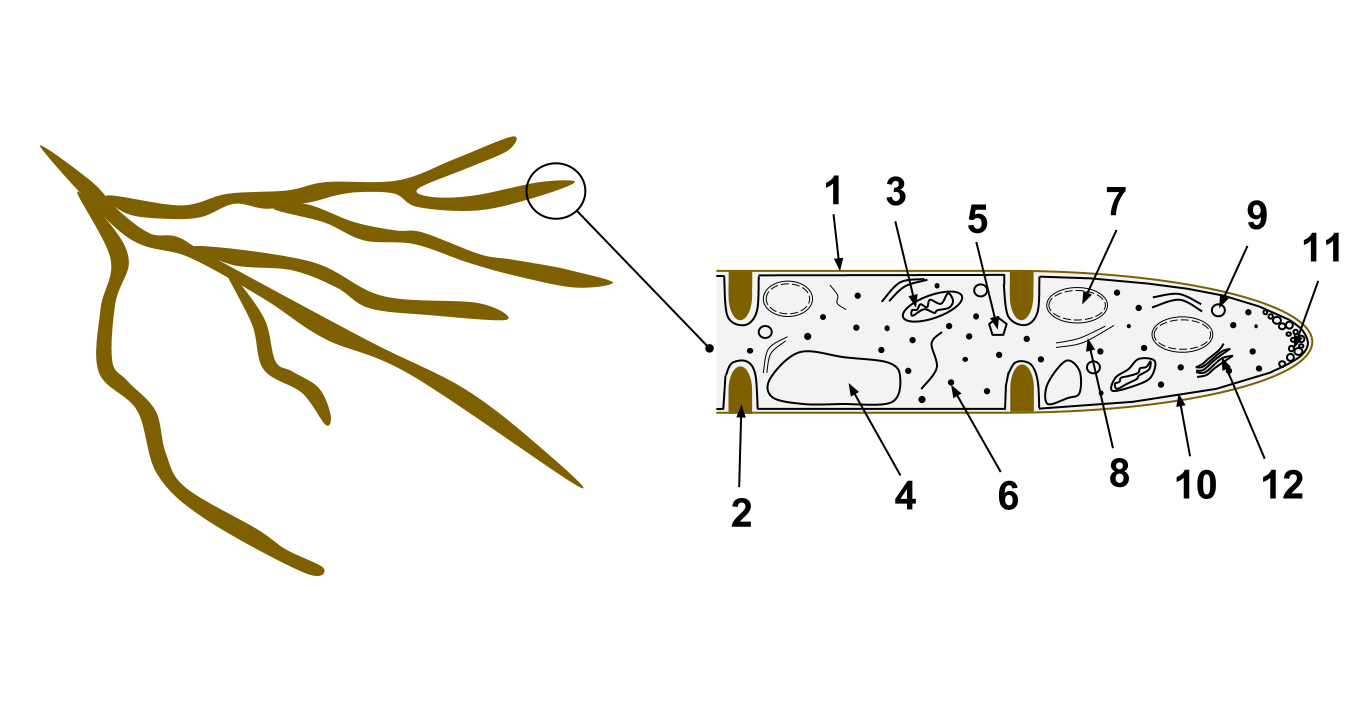
\includegraphics[width=0.7\linewidth]{./figures/fungi/HYPHAE} 

}

\caption{\href{https://commons.wikimedia.org/wiki/File:HYPHAE.png}{Fungal hyphae cells} 1. Hyphal wall 2. Septum 3. Mitochondrion 4. Vacuole 5. Ergosterol crystal 6. Ribosome 7. Nucleus 8. Endoplasmic reticulum 9. Lipid body 10. Plasma membrane 11. Spitzenkörper 12. Golgi apparatus}\label{fig:hyphaecell}
\end{figure}

Unique features of fungi:

\begin{itemize}
\tightlist
\item
  Some species grow as unicellular yeasts that reproduce by budding or fission. Dimorphic fungi can switch between a yeast phase and a hyphal phase in response to environmental conditions.
\item
  The fungal cell wall is composed of glucans and chitin; while glucans are also found in plants and chitin in the exoskeleton of arthropods, fungi are the only organisms that combine these two structural molecules in their cell wall. Unlike those of plants and oomycetes, fungal cell walls do not contain cellulose.
\end{itemize}

Most fungi lack an efficient system for the long-distance transport of water and nutrients, such as the xylem and phloem in many plants. To overcome this limitation, some fungi, such as Armillaria, form rhizomorphs, which resemble and perform functions similar to the roots of plants. As eukaryotes, fungi possess a biosynthetic pathway for producing terpenes that uses mevalonic acid and pyrophosphate as chemical building blocks. Plants and some other organisms have an additional terpene biosynthesis pathway in their chloroplasts, a structure fungi and animals do not have. Fungi produce several secondary metabolites that are similar or identical in structure to those made by plants. Many of the plant and fungal enzymes that make these compounds differ from each other in sequence and other characteristics, which indicates separate origins and convergent evolution of these enzymes in the fungi and plants.

Fungi have a worldwide distribution, and grow in a wide range of habitats, including extreme environments such as deserts or areas with high salt concentrations or ionizing radiation, as well as in deep sea sediments. Some can survive the intense UV and cosmic radiation encountered during space travel. Most grow in terrestrial environments, though several species live partly or solely in aquatic habitats, such as the chytrid fungus Batrachochytrium dendrobatidis, a parasite that has been responsible for a worldwide decline in amphibian populations. This organism spends part of its life cycle as a motile zoospore, enabling it to propel itself through water and enter its amphibian host. Other examples of aquatic fungi include those living in hydrothermal areas of the ocean.

Around 120,000 species of fungi have been described by taxonomists, but the global biodiversity of the fungus kingdom is not fully understood. A 2017 estimate suggests there may be between 2.2 and 3.8 million species. In mycology, species have historically been distinguished by a variety of methods and concepts. Classification based on morphological characteristics, such as the size and shape of spores or fruiting structures, has traditionally dominated fungal taxonomy. Species may also be distinguished by their biochemical and physiological characteristics, such as their ability to metabolize certain biochemicals, or their reaction to chemical tests. The biological species concept discriminates species based on their ability to mate. The application of molecular tools, such as DNA sequencing and phylogenetic analysis, to study diversity has greatly enhanced the resolution and added robustness to estimates of genetic diversity within various taxonomic groups.

\hypertarget{morphology-of-fungi}{%
\section{Morphology of Fungi}\label{morphology-of-fungi}}

Most fungi grow as hyphae, which are cylindrical, thread-like structures 2--10 µm in diameter and up to several centimeters in length. Hyphae grow at their tips (apices); new hyphae are typically formed by emergence of new tips along existing hyphae by a process called branching, or occasionally growing hyphal tips fork, giving rise to two parallel-growing hyphae. Hyphae also sometimes fuse when they come into contact, a process called hyphal fusion (or anastomosis). These growth processes lead to the development of a mycelium, an interconnected network of hyphae. Hyphae can be either septate or coenocytic. Septate hyphae are divided into compartments separated by cross walls (internal cell walls, called septa, that are formed at right angles to the cell wall giving the hypha its shape), with each compartment containing one or more nuclei; coenocytic hyphae are not compartmentalized. Septa have pores that allow cytoplasm, organelles, and sometimes nuclei to pass through; an example is the dolipore septum in fungi of the phylum Basidiomycota. Coenocytic hyphae are in essence multinucleate supercells.

Many species have developed specialized hyphal structures for nutrient uptake from living hosts; examples include haustoria in plant-parasitic species of most fungal phyla, and arbuscules of several mycorrhizal fungi, which penetrate into the host cells to consume nutrients.

Although fungi are opisthokonts---a grouping of evolutionarily related organisms broadly characterized by a single posterior flagellum---all phyla except for the chytrids have lost their posterior flagella. Fungi are unusual among the eukaryotes in having a cell wall that, in addition to glucans (e.g., β-1,3-glucan) and other typical components, also contains the biopolymer chitin.

Fungal mycelia can become visible to the naked eye, for example, on various surfaces and substrates, such as damp walls and spoiled food, where they are commonly called molds. Mycelia grown on solid agar media in laboratory petri dishes are usually referred to as colonies. These colonies can exhibit growth shapes and colors (due to spores or pigmentation) that can be used as diagnostic features in the identification of species or groups. Some individual fungal colonies can reach extraordinary dimensions and ages as in the case of a clonal colony of Armillaria solidipes, which extends over an area of more than 900 ha (3.5 square miles), with an estimated age of nearly 9,000 years.

The apothecium---a specialized structure important in sexual reproduction in the ascomycetes---is a cup-shaped fruit body that is often macroscopic and holds the hymenium, a layer of tissue containing the spore-bearing cells. The fruit bodies of the basidiomycetes (basidiocarps) and some ascomycetes can sometimes grow very large, and many are well known as mushrooms.

\hypertarget{growth-and-physiology-of-fungi}{%
\section{Growth And Physiology of Fungi}\label{growth-and-physiology-of-fungi}}

The growth of fungi as hyphae on or in solid substrates or as single cells in aquatic environments is adapted for the efficient extraction of nutrients, because these growth forms have high surface area to volume ratios. Hyphae are specifically adapted for growth on solid surfaces, and to invade substrates and tissues. They can exert large penetrative mechanical forces; for example, many plant pathogens, including Magnaporthe grisea, form a structure called an appressorium that evolved to puncture plant tissues. The pressure generated by the appressorium, directed against the plant epidermis, can exceed 8 megapascals (1,200 psi). The filamentous fungus Paecilomyces lilacinus uses a similar structure to penetrate the eggs of nematodes.

The mechanical pressure exerted by the appressorium is generated from physiological processes that increase intracellular turgor by producing osmolytes such as glycerol. Adaptations such as these are complemented by hydrolytic enzymes secreted into the environment to digest large organic molecules---such as polysaccharides, proteins, and lipids---into smaller molecules that may then be absorbed as nutrients. The vast majority of filamentous fungi grow in a polar fashion (extending in one direction) by elongation at the tip (apex) of the hypha. Other forms of fungal growth include intercalary extension (longitudinal expansion of hyphal compartments that are below the apex) as in the case of some endophytic fungi, or growth by volume expansion during the development of mushroom stipes and other large organs. Growth of fungi as multicellular structures consisting of somatic and reproductive cells---a feature independently evolved in animals and plants---has several functions, including the development of fruit bodies for dissemination of sexual spores (see above) and biofilms for substrate colonization and intercellular communication.

The fungi are traditionally considered heterotrophs, organisms that rely solely on carbon fixed by other organisms for metabolism. Fungi have evolved a high degree of metabolic versatility that allows them to use a diverse range of organic substrates for growth, including simple compounds such as nitrate, ammonia, acetate, or ethanol. In some species the pigment melanin may play a role in extracting energy from ionizing radiation, such as gamma radiation. This form of ``radiotrophic'' growth has been described for only a few species, the effects on growth rates are small, and the underlying biophysical and biochemical processes are not well known. This process might bear similarity to CO\textsubscript{2}fixation via visible light, but instead uses ionizing radiation as a source of energy.

\hypertarget{reproduction-of-fungi}{%
\section{Reproduction of Fungi}\label{reproduction-of-fungi}}

Fungal reproduction is complex, reflecting the differences in lifestyles and genetic makeup within this diverse kingdom of organisms. It is estimated that a third of all fungi reproduce using more than one method of propagation; for example, reproduction may occur in two well-differentiated stages within the life cycle of a species, the teleomorph and the anamorph. Environmental conditions trigger genetically determined developmental states that lead to the creation of specialized structures for sexual or asexual reproduction. These structures aid reproduction by efficiently dispersing spores or spore-containing propagules.

\hypertarget{asexual-reproduction}{%
\subsection{Asexual reproduction}\label{asexual-reproduction}}

Asexual reproduction occurs via vegetative spores (conidia) or through mycelial fragmentation. Mycelial fragmentation occurs when a fungal mycelium separates into pieces, and each component grows into a separate mycelium. Mycelial fragmentation and vegetative spores maintain clonal populations adapted to a specific niche, and allow more rapid dispersal than sexual reproduction. The ``Fungi imperfecti'' (fungi lacking the perfect or sexual stage) or Deuteromycota comprise all the species that lack an observable sexual cycle. Deuteromycota is not an accepted taxonomic clade, and is now taken to mean simply fungi that lack a known sexual stage.

\hypertarget{sexual-reproduction-1}{%
\subsection{Sexual reproduction}\label{sexual-reproduction-1}}

Sexual reproduction with meiosis has been directly observed in all fungal phyla except Glomeromycota (genetic analysis suggests meiosis in Glomeromycota as well). It differs in many aspects from sexual reproduction in animals or plants. Differences also exist between fungal groups and can be used to discriminate species by morphological differences in sexual structures and reproductive strategies. Mating experiments between fungal isolates may identify species on the basis of biological species concepts. The major fungal groupings have initially been delineated based on the morphology of their sexual structures and spores; for example, the spore-containing structures, asci and basidia, can be used in the identification of ascomycetes and basidiomycetes, respectively. Fungi employ two mating systems: heterothallic species allow mating only between individuals of opposite mating type, whereas homothallic species can mate, and sexually reproduce, with any other individual or itself.

Most fungi have both a haploid and a diploid stage in their life cycles. In sexually reproducing fungi, compatible individuals may combine by fusing their hyphae together into an interconnected network; this process, anastomosis, is required for the initiation of the sexual cycle. Many ascomycetes and basidiomycetes go through a dikaryotic stage, in which the nuclei inherited from the two parents do not combine immediately after cell fusion, but remain separate in the hyphal cells (see heterokaryosis).

In ascomycetes, dikaryotic hyphae of the hymenium (the spore-bearing tissue layer) form a characteristic hook at the hyphal septum. During cell division, formation of the hook ensures proper distribution of the newly divided nuclei into the apical and basal hyphal compartments. An ascus (plural asci) is then formed, in which karyogamy (nuclear fusion) occurs. Asci are embedded in an ascocarp, or fruiting body. Karyogamy in the asci is followed immediately by meiosis and the production of ascospores. After dispersal, the ascospores may germinate and form a new haploid mycelium.

Sexual reproduction in basidiomycetes is similar to that of the ascomycetes. Compatible haploid hyphae fuse to produce a dikaryotic mycelium. However, the dikaryotic phase is more extensive in the basidiomycetes, often also present in the vegetatively growing mycelium. A specialized anatomical structure, called a clamp connection, is formed at each hyphal septum. As with the structurally similar hook in the ascomycetes, the clamp connection in the basidiomycetes is required for controlled transfer of nuclei during cell division, to maintain the dikaryotic stage with two genetically different nuclei in each hyphal compartment. A basidiocarp is formed in which club-like structures known as basidia generate haploid basidiospores after karyogamy and meiosis. The most commonly known basidiocarps are mushrooms, but they may also take other forms (see Morphology section).

In fungi formerly classified as Zygomycota, haploid hyphae of two individuals fuse, forming a gametangium, a specialized cell structure that becomes a fertile gamete-producing cell. The gametangium develops into a zygospore, a thick-walled spore formed by the union of gametes. When the zygospore germinates, it undergoes meiosis, generating new haploid hyphae, which may then form asexual sporangiospores. These sporangiospores allow the fungus to rapidly disperse and germinate into new genetically identical haploid fungal mycelia.

\hypertarget{spore-dispersal}{%
\subsection{Spore dispersal}\label{spore-dispersal}}

Both asexual and sexual spores or sporangiospores are often actively dispersed by forcible ejection from their reproductive structures. This ejection ensures exit of the spores from the reproductive structures as well as traveling through the air over long distances.

Specialized mechanical and physiological mechanisms, as well as spore surface structures (such as hydrophobins), enable efficient spore ejection. For example, the structure of the spore-bearing cells in some ascomycete species is such that the buildup of substances affecting cell volume and fluid balance enables the explosive discharge of spores into the air. The forcible discharge of single spores termed ballistospores involves formation of a small drop of water (Buller's drop), which upon contact with the spore leads to its projectile release with an initial acceleration of more than 10,000 g; the net result is that the spore is ejected 0.01--0.02 cm, sufficient distance for it to fall through the gills or pores into the air below. Other fungi, like the puffballs, rely on alternative mechanisms for spore release, such as external mechanical forces. The hydnoid fungi (tooth fungi) produce spores on pendant, tooth-like or spine-like projections. The bird's nest fungi use the force of falling water drops to liberate the spores from cup-shaped fruiting bodies. Another strategy is seen in the stinkhorns, a group of fungi with lively colors and putrid odor that attract insects to disperse their spores.

The most common means of spore dispersal is by wind - species using this form of dispersal often produce dry or hydrophobic spores which do not absorb water and are readily scattered by raindrops, for example. Most of the researched species of fungus are transported by wind.

\hypertarget{evolution-of-fungi}{%
\section{Evolution of Fungi}\label{evolution-of-fungi}}

In contrast to plants and animals, the early fossil record of the fungi is meager. The earliest fossils possessing features typical of fungi date to the Paleoproterozoic era, some 2,400 million years ago (Ma); these multicellular benthic organisms had filamentous structures capable of anastomosis. Other studies (2009) estimate the arrival of fungal organisms at about 760--1060 Ma on the basis of comparisons of the rate of evolution in closely related groups. For much of the Paleozoic Era (542--251 Ma), the fungi appear to have been aquatic and consisted of organisms similar to the extant chytrids in having flagellum-bearing spores. The evolutionary adaptation from an aquatic to a terrestrial lifestyle necessitated a diversification of ecological strategies for obtaining nutrients, including parasitism, saprobism, and the development of mutualistic relationships such as mycorrhiza and lichenization. Recent (2009) studies suggest that the ancestral ecological state of the Ascomycota was saprobism, and that independent lichenization events have occurred multiple times.

In May 2019, scientists reported the discovery of a fossilized fungus, named Ourasphaira giraldae, in the Canadian Arctic, that may have grown on land a billion years ago, well before plants were living on land. Earlier, it had been presumed that the fungi colonized the land during the Cambrian (542--488.3 Ma), also long before land plants. Fossilized hyphae and spores recovered from the Ordovician of Wisconsin (460 Ma) resemble modern-day Glomerales, and existed at a time when the land flora likely consisted of only non-vascular bryophyte-like plants. Prototaxites, which was probably a fungus or lichen, would have been the tallest organism of the late Silurian and early Devonian. Fungal fossils do not become common and uncontroversial until the early Devonian (416--359.2 Ma), when they occur abundantly in the Rhynie chert, mostly as Zygomycota and Chytridiomycota. At about this same time, approximately 400 Ma, the Ascomycota and Basidiomycota diverged, and all modern classes of fungi were present by the Late Carboniferous (Pennsylvanian, 318.1--299 Ma).

Lichen-like fossils have been found in the Doushantuo Formation in southern China dating back to 635--551 Ma. Lichens formed a component of the early terrestrial ecosystems, and the estimated age of the oldest terrestrial lichen fossil is 400 Ma; this date corresponds to the age of the oldest known sporocarp fossil, a Paleopyrenomycites species found in the Rhynie Chert. The oldest fossil with microscopic features resembling modern-day basidiomycetes is Palaeoancistrus, found permineralized with a fern from the Pennsylvanian. Rare in the fossil record are the Homobasidiomycetes (a taxon roughly equivalent to the mushroom-producing species of the Agaricomycetes). Two amber-preserved specimens provide evidence that the earliest known mushroom-forming fungi (the extinct species Archaeomarasmius leggetti) appeared during the late Cretaceous, 90 Ma.

Some time after the Permian--Triassic extinction event (251.4 Ma), a fungal spike (originally thought to be an extraordinary abundance of fungal spores in sediments) formed, suggesting that fungi were the dominant life form at this time, representing nearly 100\% of the available fossil record for this period. However, the relative proportion of fungal spores relative to spores formed by algal species is difficult to assess, the spike did not appear worldwide, and in many places it did not fall on the Permian--Triassic boundary.

65 million years ago, immediately after the Cretaceous--Paleogene extinction event that famously killed off most dinosaurs, there is a dramatic increase in evidence of fungi, apparently the death of most plant and animal species leading to a huge fungal bloom like ``a massive compost heap''.

Although commonly included in botany curricula and textbooks, fungi are more closely related to animals than to plants and are placed with the animals in the monophyletic group of opisthokonts. Analyses using molecular phylogenetics support a monophyletic origin of fungi. The taxonomy of fungi is in a state of constant flux, especially due to recent research based on DNA comparisons. These current phylogenetic analyses often overturn classifications based on older and sometimes less discriminative methods based on morphological features and biological species concepts obtained from experimental matings.

There is no unique generally accepted system at the higher taxonomic levels and there are frequent name changes at every level, from species upwards. Efforts among researchers are now underway to establish and encourage usage of a unified and more consistent nomenclature. Fungal species can also have multiple scientific names depending on their life cycle and mode (sexual or asexual) of reproduction. Web sites such as Index Fungorum and ITIS list current names of fungal species (with cross-references to older synonyms).

The 2007 classification of Kingdom Fungi is the result of a large-scale collaborative research effort involving dozens of mycologists and other scientists working on fungal taxonomy. It recognizes seven phyla, two of which---the Ascomycota and the Basidiomycota---are contained within a branch representing subkingdom Dikarya, the most species rich and familiar group, including all the mushrooms, most food-spoilage molds, most plant pathogenic fungi, and the beer, wine, and bread yeasts.

The major phyla (sometimes called divisions) of fungi have been classified mainly on the basis of characteristics of their sexual reproductive structures.



\begin{figure}

{\centering 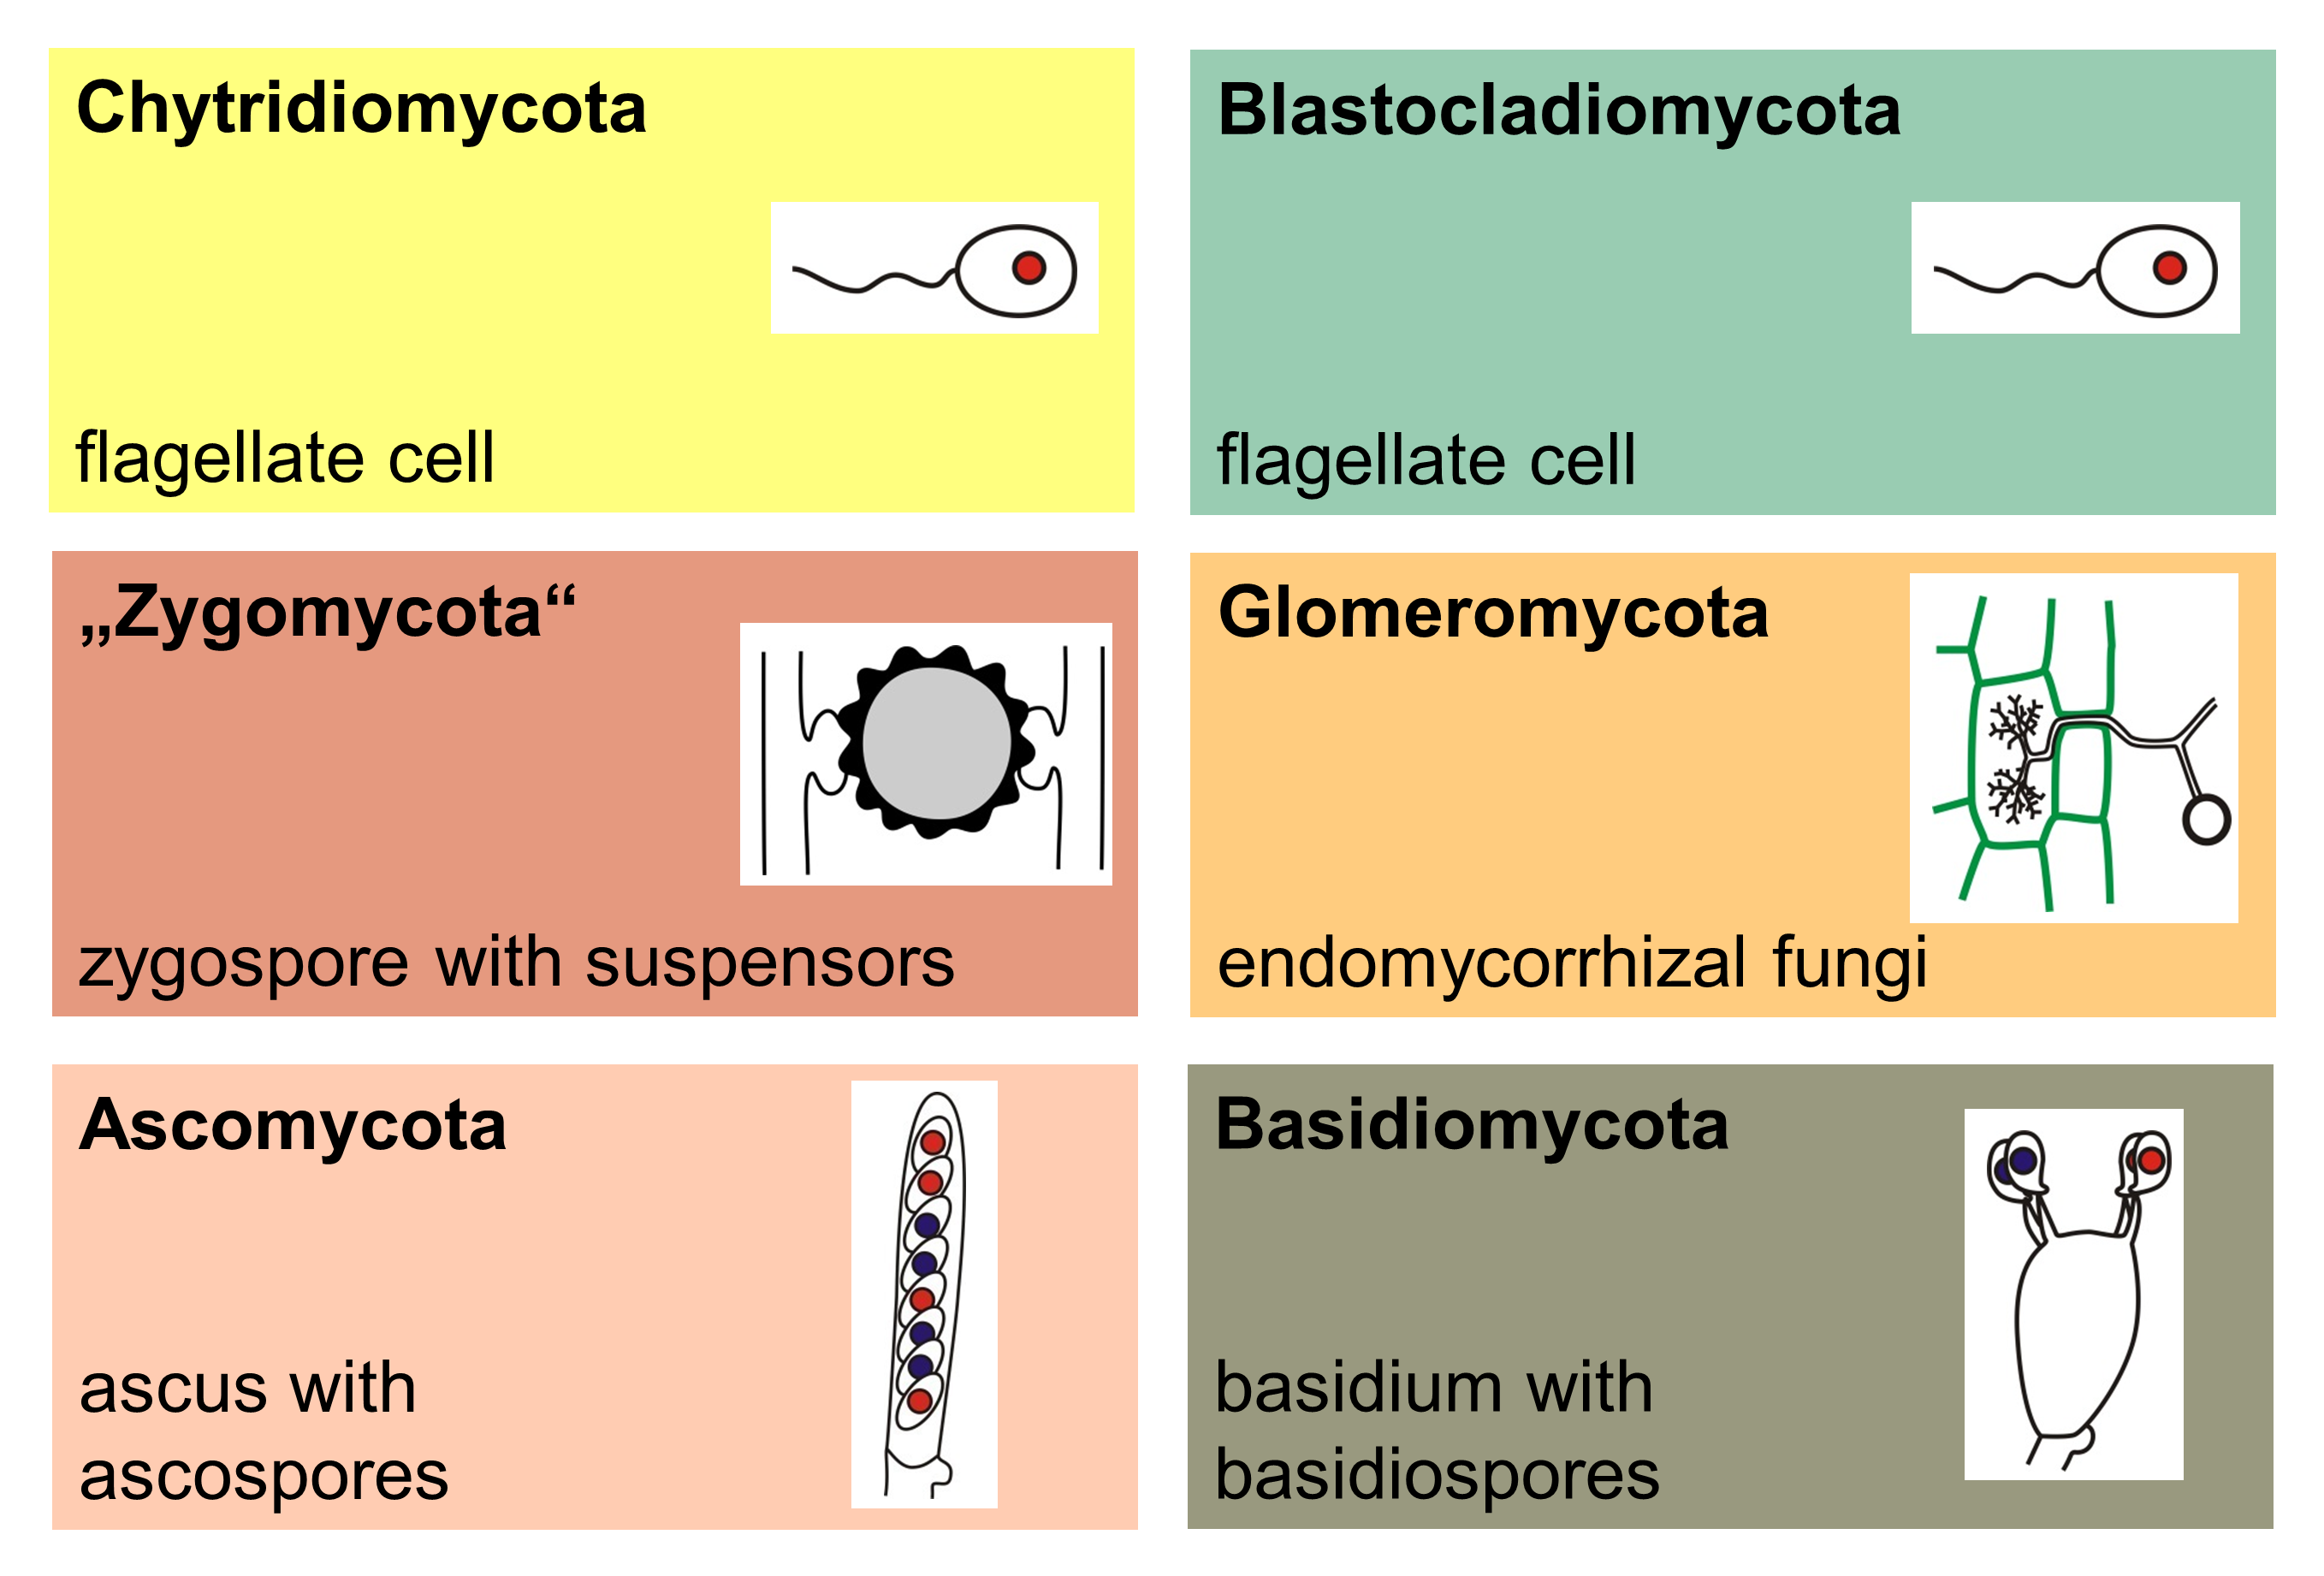
\includegraphics[width=0.7\linewidth]{./figures/fungi/02_01_groups_of_Fungi_(M._Piepenbring)} 

}

\caption{\href{https://commons.wikimedia.org/wiki/File:02_01_groups_of_Fungi_(M._Piepenbring).png}{Six commonly recognized groups of fungi.} Zygomycota, or zygote fungi, is a former division or phylum of the kingdom Fungi. The members are now part of two recently proposed phyla.}\label{fig:fungitaxonomy}
\end{figure}

Phylogenetic analysis has demonstrated that the Microsporidia, unicellular parasites of animals and protists, are fairly recent and highly derived endobiotic fungi (living within the tissue of another species). One 2006 study concludes that the Microsporidia are a sister group to the true fungi; that is, they are each other's closest evolutionary relative. Hibbett and colleagues suggest that this analysis does not clash with their classification of the Fungi, and although the Microsporidia are elevated to phylum status, it is acknowledged that further analysis is required to clarify evolutionary relationships within this group.

The Chytridiomycota are commonly known as chytrids. These fungi are distributed worldwide. Chytrids and their close relatives Neocallimastigomycota and Blastocladiomycota (below) are the only fungi with active motility, producing zoospores that are capable of active movement through aqueous phases with a single flagellum, leading early taxonomists to classify them as protists. Molecular phylogenies, inferred from rRNA sequences in ribosomes, suggest that the Chytrids are a basal group divergent from the other fungal phyla, consisting of four major clades with suggestive evidence for paraphyly or possibly polyphyly.

The Blastocladiomycota were previously considered a taxonomic clade within the Chytridiomycota. Recent molecular data and ultrastructural characteristics, however, place the Blastocladiomycota as a sister clade to the Zygomycota, Glomeromycota, and Dikarya (Ascomycota and Basidiomycota). The blastocladiomycetes are saprotrophs, feeding on decomposing organic matter, and they are parasites of all eukaryotic groups. Unlike their close relatives, the chytrids, most of which exhibit zygotic meiosis, the blastocladiomycetes undergo sporic meiosis.

The Neocallimastigomycota were earlier placed in the phylum Chytridomycota. Members of this small phylum are anaerobic organisms, living in the digestive system of larger herbivorous mammals and in other terrestrial and aquatic environments enriched in cellulose (e.g., domestic waste landfill sites). They lack mitochondria but contain hydrogenosomes of mitochondrial origin. As in the related chrytrids, neocallimastigomycetes form zoospores that are posteriorly uniflagellate or polyflagellate.

Members of the Glomeromycota form arbuscular mycorrhizae, a form of mutualist symbiosis wherein fungal hyphae invade plant root cells and both species benefit from the resulting increased supply of nutrients. All known Glomeromycota species reproduce asexually. The symbiotic association between the Glomeromycota and plants is ancient, with evidence dating to 400 million years ago. Formerly part of the Zygomycota (commonly known as `sugar' and `pin' molds), the Glomeromycota were elevated to phylum status in 2001 and now replace the older phylum Zygomycota. Fungi that were placed in the Zygomycota are now being reassigned to the Glomeromycota, or the subphyla incertae sedis Mucoromycotina, Kickxellomycotina, the Zoopagomycotina and the Entomophthoromycotina. Some well-known examples of fungi formerly in the Zygomycota include black bread mold (Rhizopus stolonifer), and Pilobolus species, capable of ejecting spores several meters through the air. Medically relevant genera include Mucor, Rhizomucor, and Rhizopus.

The Ascomycota, commonly known as sac fungi or ascomycetes, constitute the largest taxonomic group within the Eumycota. These fungi form meiotic spores called ascospores, which are enclosed in a special sac-like structure called an ascus. This phylum includes morels, a few mushrooms and truffles, unicellular yeasts (e.g., of the genera Saccharomyces, Kluyveromyces, Pichia, and Candida), and many filamentous fungi living as saprotrophs, parasites, and mutualistic symbionts (e.g.~lichens). Prominent and important genera of filamentous ascomycetes include Aspergillus, Penicillium, Fusarium, and Claviceps. Many ascomycete species have only been observed undergoing asexual reproduction (called anamorphic species), but analysis of molecular data has often been able to identify their closest teleomorphs in the Ascomycota. Because the products of meiosis are retained within the sac-like ascus, ascomycetes have been used for elucidating principles of genetics and heredity (e.g., Neurospora crassa).



\begin{figure}

{\centering 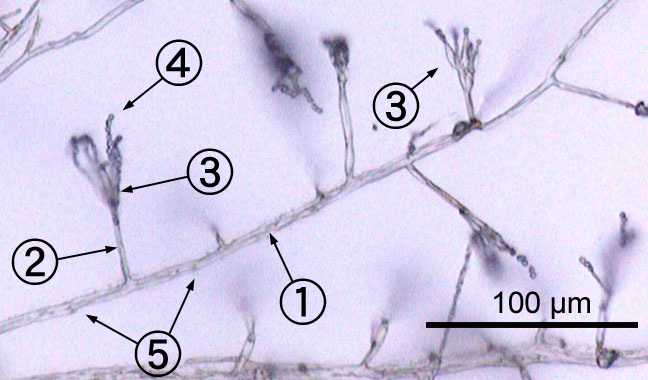
\includegraphics[width=0.7\linewidth]{./figures/fungi/Penicillium_labeled_cropped} 

}

\caption{\href{https://commons.wikimedia.org/wiki/File:Penicillium_labeled_cropped.jpg}{An environmental isolate of Penicillium hypha conidiophore phialide conidia septa} 1. hypha 2. conidiophore 3. phialide 4. conidia 5. septa}\label{fig:penicillium}
\end{figure}

Members of the Basidiomycota, commonly known as the club fungi or basidiomycetes, produce meiospores called basidiospores on club-like stalks called basidia. Most common mushrooms belong to this group, as well as rust and smut fungi, which are major pathogens of grains. Other important basidiomycetes include the maize pathogen Ustilago maydis, human commensal species of the genus Malassezia, and the opportunistic human pathogen, Cryptococcus neoformans.

\hypertarget{fungus-like-organisms}{%
\section{Fungus-like organisms}\label{fungus-like-organisms}}

Because of similarities in morphology and lifestyle, the slime molds, water molds (oomycetes) and hyphochytrids (both Stramenopiles) were formerly classified in the kingdom Fungi.

Unlike true fungi, the cell walls of oomycetes contain cellulose and lack chitin. Hyphochytrids have both chitin and cellulose. Slime molds lack a cell wall during the assimilative phase (except labyrinthulids, which have a wall of scales), and ingest nutrients by ingestion (phagocytosis, except labyrinthulids) rather than absorption (osmotrophy, as fungi, labyrinthulids, oomycetes and hyphochytrids). Neither water molds nor slime molds are closely related to the true fungi, and, therefore, taxonomists no longer group them in the kingdom Fungi. Nonetheless, studies of the oomycetes and myxomycetes are still often included in mycology textbooks and primary research literature.

\hypertarget{ecology-of-fungi}{%
\section{Ecology of Fungi}\label{ecology-of-fungi}}

Although often inconspicuous, fungi occur in every environment on Earth and play very important roles in most ecosystems. Along with bacteria, fungi are the major decomposers in most terrestrial (and some aquatic) ecosystems, and therefore play a critical role in biogeochemical cycles and in many food webs. As decomposers, they play an essential role in nutrient cycling, especially as saprotrophs and symbionts, degrading organic matter to inorganic molecules, which can then re-enter anabolic metabolic pathways in plants or other organisms.

\hypertarget{symbiosis}{%
\subsection{Symbiosis}\label{symbiosis}}

Many fungi have important symbiotic relationships with organisms from most if not all kingdoms. These interactions can be mutualistic or antagonistic in nature, or in the case of commensal fungi are of no apparent benefit or detriment to the host.

Mycorrhizal symbiosis between plants and fungi is one of the most well-known plant--fungus associations and is of significant importance for plant growth and persistence in many ecosystems; over 90\% of all plant species engage in mycorrhizal relationships with fungi and are dependent upon this relationship for survival.



\begin{figure}

{\centering 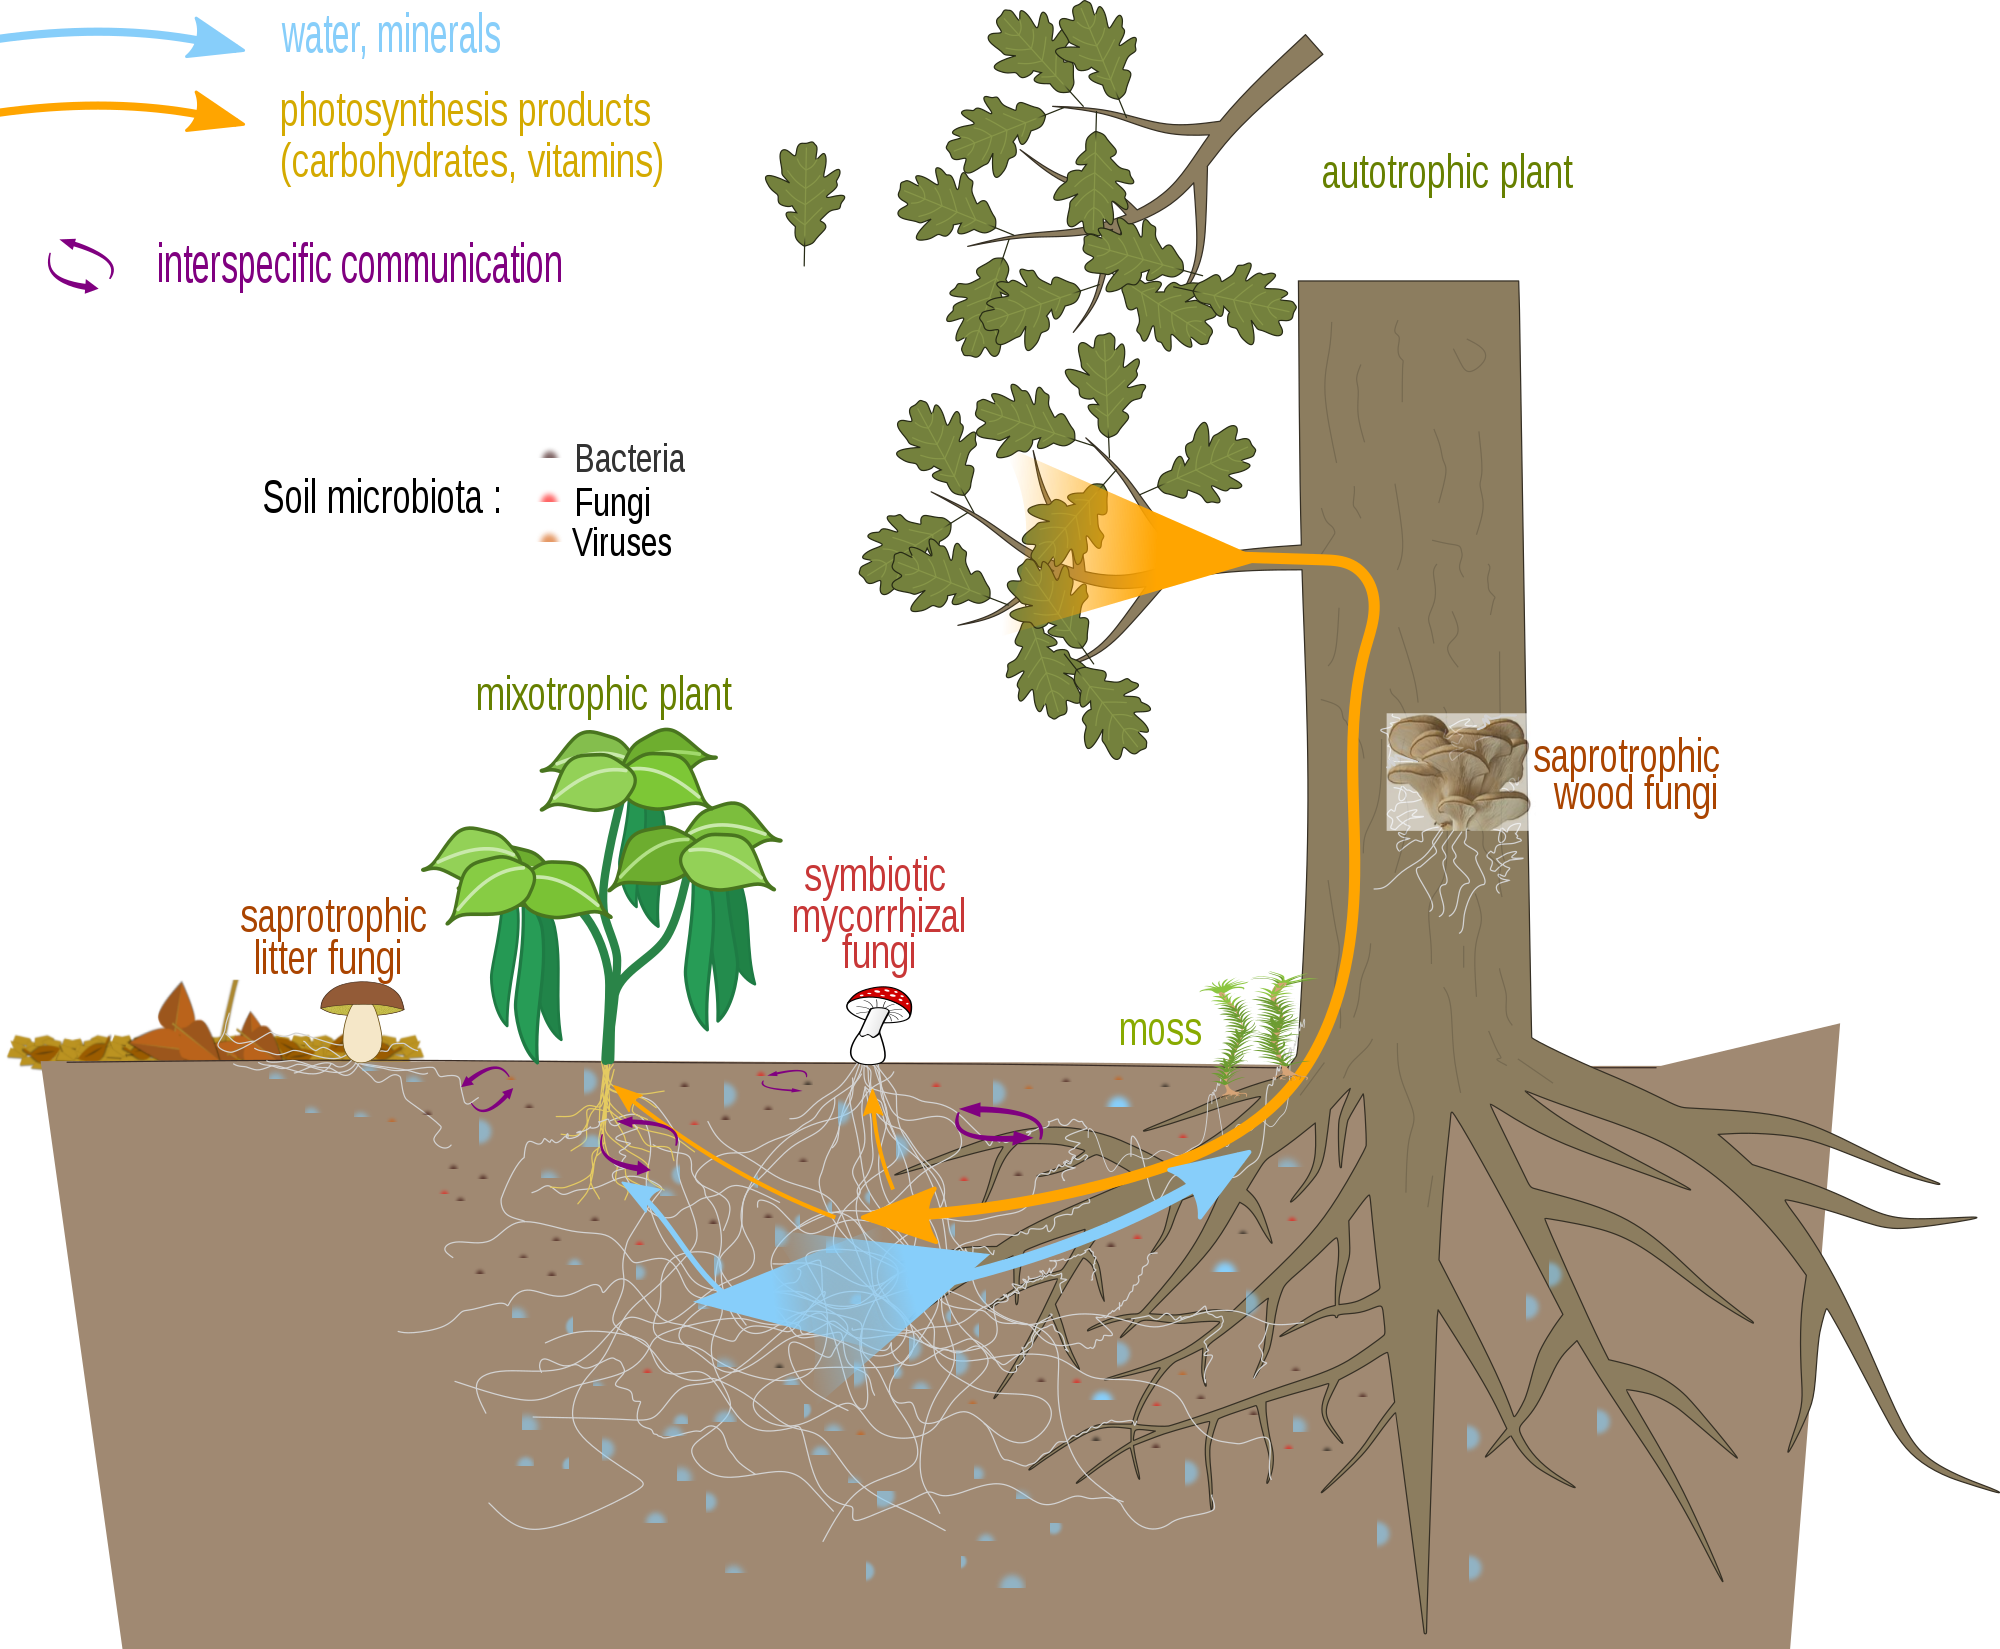
\includegraphics[width=0.7\linewidth]{./figures/fungi/Mycorrhizal_network} 

}

\caption{\href{https://commons.wikimedia.org/wiki/File:Mycorrhizal_network.svg}{Nutrient exchanges and communication between a mycorrhizal fungus and plants.}}\label{fig:mycorhiza}
\end{figure}

The mycorrhizal symbiosis is ancient, dating to at least 400 million years ago. It often increases the plant's uptake of inorganic compounds, such as nitrate and phosphate from soils having low concentrations of these key plant nutrients. The fungal partners may also mediate plant-to-plant transfer of carbohydrates and other nutrients. Such mycorrhizal communities are called ``common mycorrhizal networks''. A special case of mycorrhiza is myco-heterotrophy, whereby the plant parasitizes the fungus, obtaining all of its nutrients from its fungal symbiont. Some fungal species inhabit the tissues inside roots, stems, and leaves, in which case they are called endophytes. Similar to mycorrhiza, endophytic colonization by fungi may benefit both symbionts; for example, endophytes of grasses impart to their host increased resistance to herbivores and other environmental stresses and receive food and shelter from the plant in return.

Lichens are a symbiotic relationship between fungi and photosynthetic algae or cyanobacteria. The photosynthetic partner in the relationship is referred to in lichen terminology as a ``photobiont''.



\begin{figure}

{\centering 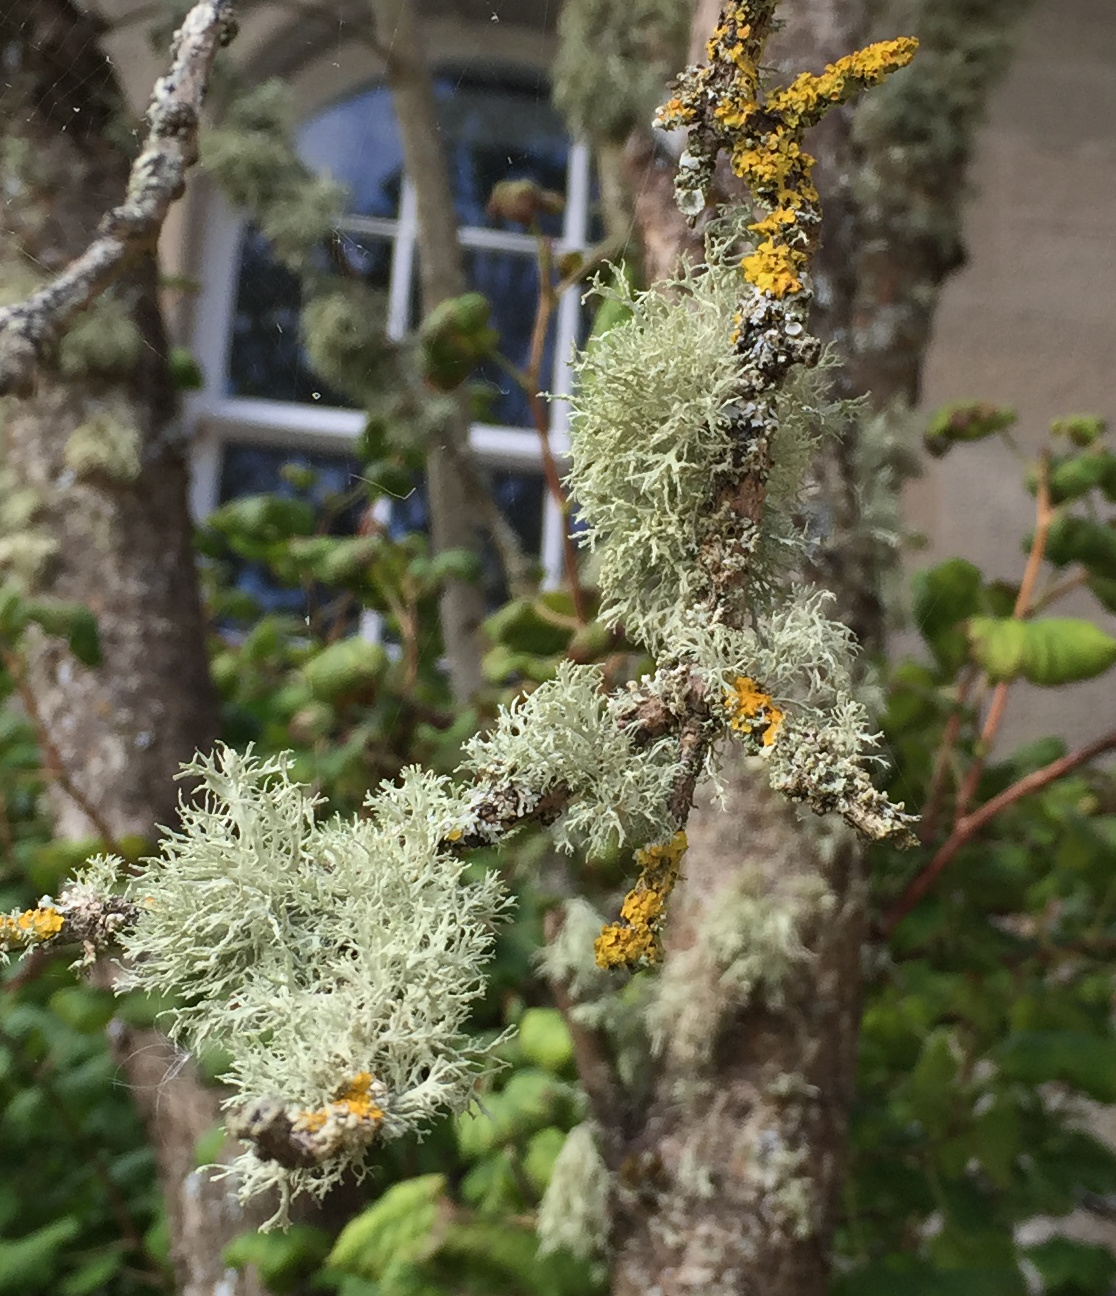
\includegraphics[width=0.7\linewidth]{./figures/fungi/lichen} 

}

\caption{Fruticose (light green) and crustose (yellow) lichens growing on a tree.}\label{fig:lichen}
\end{figure}



\begin{figure}

{\centering \includegraphics[width=0.7\linewidth]{./figures/fungi/Lichen_cross_section_–_heteromeric_thallus} 

}

\caption{\href{https://commons.wikimedia.org/wiki/File:Lichen_cross_section_–_heteromeric_thallus.svg}{Schematic cross section of foliose lichen:} a) The cortex is the outer layer of tightly woven fungus filaments (hyphae) b) This photobiont layer has photosynthesizing green algae c) Loosely packed hyphae in the medulla d) A tightly woven lower cortex e) Anchoring hyphae called rhizines where the fungus attaches to the substrate.}\label{fig:lichencrossection}
\end{figure}

The fungal part of the relationship is composed mostly of various species of ascomycetes and a few basidiomycetes.



\begin{figure}

{\centering 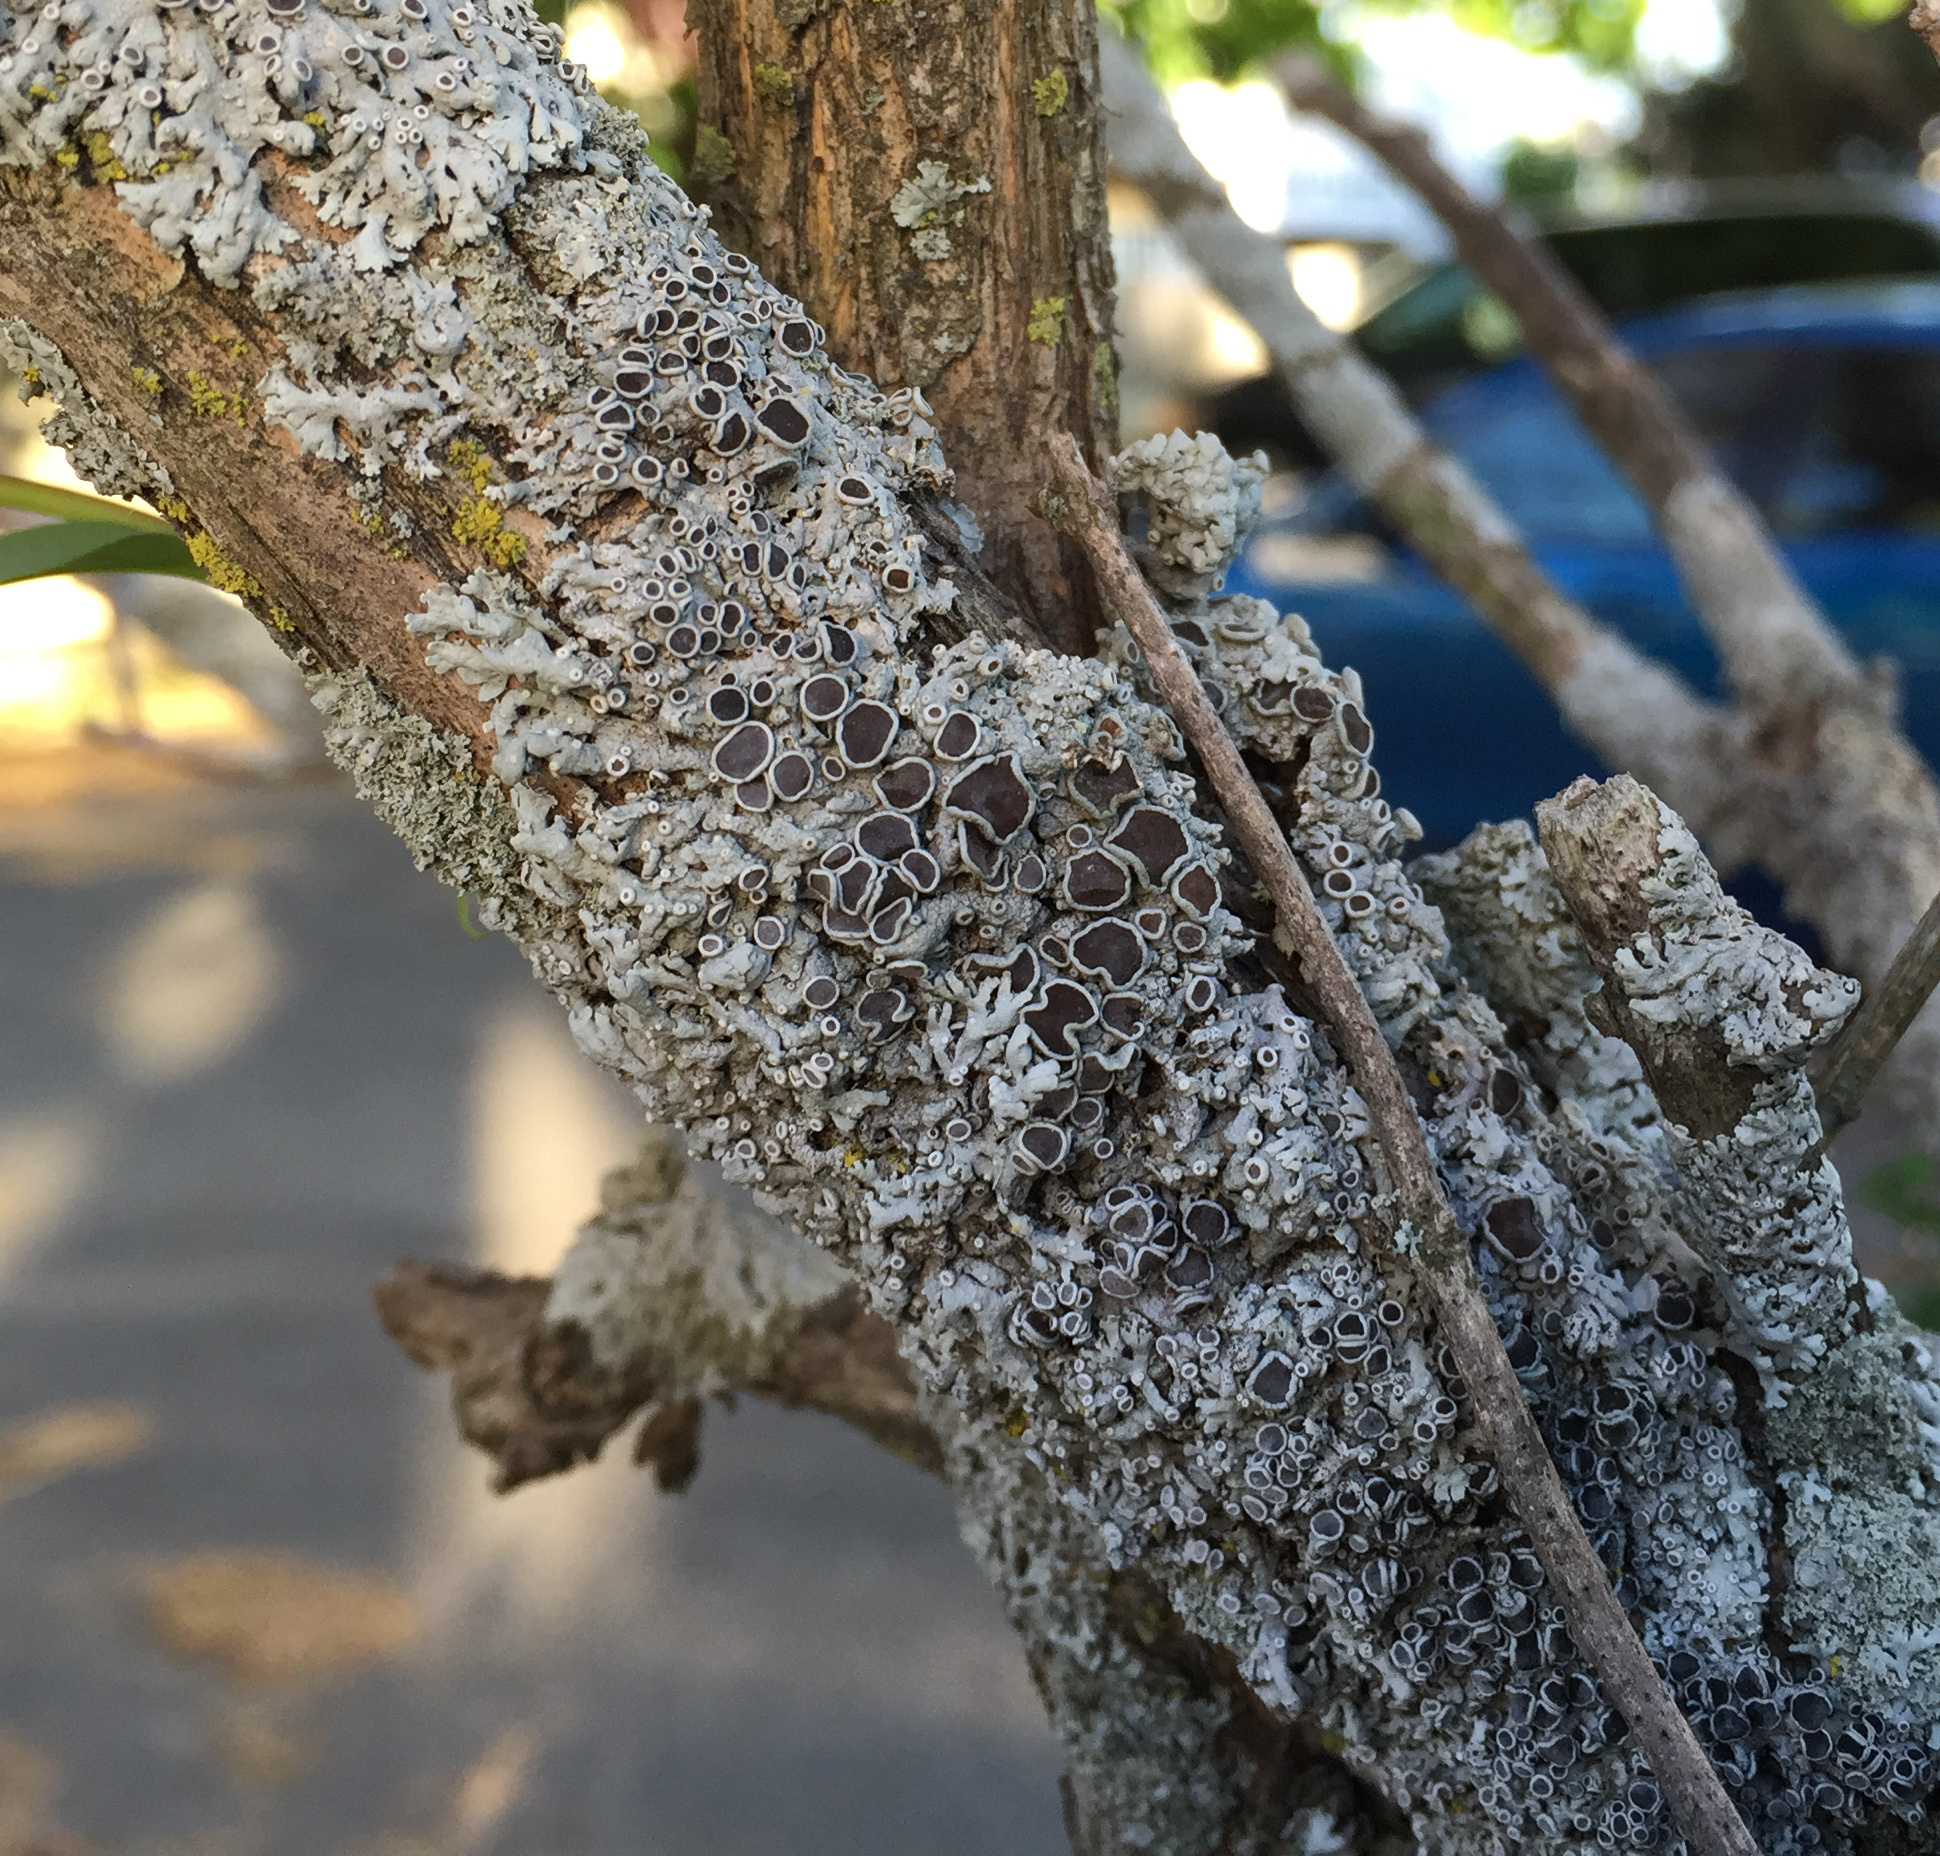
\includegraphics[width=0.7\linewidth]{./figures/fungi/lichen_apothecium} 

}

\caption{Cup-shaped apothecia and thallus of a foliose lichen.}\label{fig:lichenapothecium}
\end{figure}

Lichens occur in every ecosystem on all continents, play a key role in soil formation and the initiation of biological succession, and are prominent in some extreme environments, including polar, alpine, and semiarid desert regions. They are able to grow on inhospitable surfaces, including bare soil, rocks, tree bark, wood, shells, barnacles and leaves. As in mycorrhizas, the photobiont provides sugars and other carbohydrates via photosynthesis to the fungus, while the fungus provides minerals and water to the photobiont. The functions of both symbiotic organisms are so closely intertwined that they function almost as a single organism; in most cases the resulting organism differs greatly from the individual components. Lichenization is a common mode of nutrition for fungi; around 20\% of fungi---between 17,500 and 20,000 described species---are lichenized. Characteristics common to most lichens include obtaining organic carbon by photosynthesis, slow growth, small size, long life, long-lasting (seasonal) vegetative reproductive structures, mineral nutrition obtained largely from airborne sources, and greater tolerance of desiccation than most other photosynthetic organisms in the same habitat.

Many insects also engage in mutualistic relationships with fungi. Several groups of ants cultivate fungi in the order Agaricales as their primary food source, while ambrosia beetles cultivate various species of fungi in the bark of trees that they infest. Likewise, females of several wood wasp species (genus Sirex) inject their eggs together with spores of the wood-rotting fungus Amylostereum areolatum into the sapwood of pine trees; the growth of the fungus provides ideal nutritional conditions for the development of the wasp larvae. At least one species of stingless bee has a relationship with a fungus in the genus Monascus, where the larvae consume and depend on fungus transferred from old to new nests. Termites on the African savannah are also known to cultivate fungi, and yeasts of the genera Candida and Lachancea inhabit the gut of a wide range of insects, including neuropterans, beetles, and cockroaches; it is not known whether these fungi benefit their hosts. Fungi ingrowing dead wood are essential for xylophagous insects (e.g.~woodboring beetles). They deliver nutrients needed by xylophages to nutritionally scarce dead wood. Thanks to this nutritional enrichment the larvae of woodboring insect is able to grow and develop to adulthood. The larvae of many families of fungicolous flies, particularly those within the superfamily Sciaroidea such as the Mycetophilidae and some Keroplatidae feed on fungal fruiting bodies and sterile mycorrhizae.

\hypertarget{fungi-as-pathogens-and-parasites}{%
\section{Fungi as Pathogens And Parasites}\label{fungi-as-pathogens-and-parasites}}

Many fungi are parasites on plants, animals (including humans), and other fungi. Serious pathogens of many cultivated plants causing extensive damage and losses to agriculture and forestry include the rice blast fungus Magnaporthe oryzae, tree pathogens such as Ophiostoma ulmi and Ophiostoma novo-ulmi causing Dutch elm disease and Cryphonectria parasitica responsible for chestnut blight, and plant pathogens in the genera Fusarium, Ustilago, Alternaria, and Cochliobolus. Some carnivorous fungi, like Paecilomyces lilacinus, are predators of nematodes, which they capture using an array of specialized structures such as constricting rings or adhesive nets. Many fungi that are plant pathogens, such as Magnaporthe oryzae, can switch from being biotrophic (parasitic on living plants) to being necrotrophic (feeding on the dead tissues of plants they have killed). This same principle is applied to fungi-feeding parasites, including Asterotremella albida, which feeds on the fruit bodies of other fungi both while they are living and after they are dead.

Some fungi can cause serious diseases in humans, several of which may be fatal if untreated. These include aspergillosis, candidiasis, coccidioidomycosis, cryptococcosis, histoplasmosis, mycetomas, and paracoccidioidomycosis. Furthermore, persons with immuno-deficiencies are particularly susceptible to disease by genera such as Aspergillus, Candida, Cryptoccocus, Histoplasma, and Pneumocystis. Other fungi can attack eyes, nails, hair, and especially skin, the so-called dermatophytic and keratinophilic fungi, and cause local infections such as ringworm and athlete's foot. Fungal spores are also a cause of allergies, and fungi from different taxonomic groups can evoke allergic reactions.

The organisms which parasitize fungi are known as mycoparasitic organisms. Certain species of the genus Pythium, which are oomycetes, have potential as biocontrol agents against certain fungi. Fungi can also act as mycoparasites or antagonists of other fungi, such as Hypomyces chrysospermus, which grows on bolete mushrooms. Fungi can also become the target of infection by mycoviruses.

\hypertarget{mycotoxins}{%
\section{Mycotoxins}\label{mycotoxins}}

Many fungi produce biologically active compounds, several of which are toxic to animals or plants and are therefore called mycotoxins. Of particular relevance to humans are mycotoxins produced by molds causing food spoilage, and poisonous mushrooms (see above). Particularly infamous are the lethal amatoxins in some Amanita mushrooms, and ergot alkaloids, which have a long history of causing serious epidemics of ergotism (St Anthony's Fire) in people consuming rye or related cereals contaminated with sclerotia of the ergot fungus, Claviceps purpurea. Other notable mycotoxins include the aflatoxins, which are insidious liver toxins and highly carcinogenic metabolites produced by certain Aspergillus species often growing in or on grains and nuts consumed by humans, ochratoxins, patulin, and trichothecenes (e.g., T-2 mycotoxin) and fumonisins, which have significant impact on human food supplies or animal livestock.

Mycotoxins are secondary metabolites (or natural products), and research has established the existence of biochemical pathways solely for the purpose of producing mycotoxins and other natural products in fungi. Mycotoxins may provide fitness benefits in terms of physiological adaptation, competition with other microbes and fungi, and protection from consumption (fungivory). Many fungal secondary metabolites (or derivatives) are used medically, as described under Human Use below.

The human use of fungi for food preparation or preservation and other purposes is extensive and has a long history. Mushroom farming and mushroom gathering are large industries in many countries. The study of the historical uses and sociological impact of fungi is known as ethnomycology. Because of the capacity of this group to produce an enormous range of natural products with antimicrobial or other biological activities, many species have long been used or are being developed for industrial production of antibiotics, vitamins, and anti-cancer and cholesterol-lowering drugs. More recently, methods have been developed for genetic engineering of fungi, enabling metabolic engineering of fungal species. For example, genetic modification of yeast species---which are easy to grow at fast rates in large fermentation vessels---has opened up ways of pharmaceutical production that are potentially more efficient than production by the original source organisms.

Many species produce metabolites that are major sources of pharmacologically active drugs. Particularly important are the antibiotics, including the penicillins, a structurally related group of β-lactam antibiotics that are synthesized from small peptides. Although naturally occurring penicillins such as penicillin G (produced by Penicillium chrysogenum) have a relatively narrow spectrum of biological activity, a wide range of other penicillins can be produced by chemical modification of the natural penicillins. Modern penicillins are semisynthetic compounds, obtained initially from fermentation cultures, but then structurally altered for specific desirable properties. Other antibiotics produced by fungi include: ciclosporin, commonly used as an immunosuppressant during transplant surgery; and fusidic acid, used to help control infection from methicillin-resistant Staphylococcus aureus bacteria. Widespread use of antibiotics for the treatment of bacterial diseases, such as tuberculosis, syphilis, leprosy, and others began in the early 20th century and continues to date. In nature, antibiotics of fungal or bacterial origin appear to play a dual role: at high concentrations they act as chemical defense against competition with other microorganisms in species-rich environments, such as the rhizosphere, and at low concentrations as quorum-sensing molecules for intra- or interspecies signaling. Other drugs produced by fungi include griseofulvin isolated from Penicillium griseofulvum, used to treat fungal infections, and statins (HMG-CoA reductase inhibitors), used to inhibit cholesterol synthesis. Examples of statins found in fungi include mevastatin from Penicillium citrinum and lovastatin from Aspergillus terreus and the oyster mushroom. Fungi produce compounds that inhibit viruses and cancer cells. Specific metabolites, such as polysaccharide-K, ergotamine, and β-lactam antibiotics, are routinely used in clinical medicine. The shiitake mushroom is a source of lentinan, a clinical drug approved for use in cancer treatments in several countries, including Japan. In Europe and Japan, polysaccharide-K (brand name Krestin), a chemical derived from Trametes versicolor, is an approved adjuvant for cancer therapy.

Certain mushrooms enjoy usage as therapeutics in folk medicines, such as Traditional Chinese medicine. Notable medicinal mushrooms with a well-documented history of use include Agaricus subrufescens, Ganoderma lucidum, Psilocybe and Ophiocordyceps sinensis.

Baker's yeast or Saccharomyces cerevisiae, a unicellular fungus, is used to make bread and other wheat-based products, such as pizza dough and dumplings. Yeast species of the genus Saccharomyces are also used to produce alcoholic beverages through fermentation. Shoyu koji mold (Aspergillus oryzae) is an essential ingredient in brewing Shoyu (soy sauce) and sake, and the preparation of miso, while Rhizopus species are used for making tempeh. Several of these fungi are domesticated species that were bred or selected according to their capacity to ferment food without producing harmful mycotoxins (see below), which are produced by very closely related Aspergilli. Quorn, a meat substitute, is made from Fusarium venenatum.

Edible mushrooms include commercially raised and wild-harvested fungi. Agaricus bisporus, sold as button mushrooms when small or Portobello mushrooms when larger, is the most widely cultivated species in the West, used in salads, soups, and many other dishes. Many Asian fungi are commercially grown and have increased in popularity in the West. They are often available fresh in grocery stores and markets, including straw mushrooms (Volvariella volvacea), oyster mushrooms (Pleurotus ostreatus), shiitakes (Lentinula edodes), and enokitake (Flammulina spp.).

Many other mushroom species are harvested from the wild for personal consumption or commercial sale. Milk mushrooms, morels, chanterelles, truffles, black trumpets, and porcini mushrooms (Boletus edulis) (also known as king boletes) demand a high price on the market. They are often used in gourmet dishes.

Certain types of cheeses require inoculation of milk curds with fungal species that impart a unique flavor and texture to the cheese. Examples include the blue color in cheeses such as Stilton or Roquefort, which are made by inoculation with Penicillium roqueforti. Molds used in cheese production are non-toxic and are thus safe for human consumption; however, mycotoxins (e.g., aflatoxins, roquefortine C, patulin, or others) may accumulate because of growth of other fungi during cheese ripening or storage.

Many mushroom species are poisonous to humans and cause a range of reactions including slight digestive problems, allergic reactions, hallucinations, severe organ failure, and death. Genera with mushrooms containing deadly toxins include Conocybe, Galerina, Lepiota, and, the most infamous, Amanita. The latter genus includes the destroying angel (A. virosa) and the death cap (A. phalloides), the most common cause of deadly mushroom poisoning. The false morel (Gyromitra esculenta) is occasionally considered a delicacy when cooked, yet can be highly toxic when eaten raw. Tricholoma equestre was considered edible until it was implicated in serious poisonings causing rhabdomyolysis. Fly agaric mushrooms (Amanita muscaria) also cause occasional non-fatal poisonings, mostly as a result of ingestion for its hallucinogenic properties. Historically, fly agaric was used by different peoples in Europe and Asia and its present usage for religious or shamanic purposes is reported from some ethnic groups such as the Koryak people of northeastern Siberia.

As it is difficult to accurately identify a safe mushroom without proper training and knowledge, it is often advised to assume that a wild mushroom is poisonous and not to consume it.

In agriculture, fungi may be useful if they actively compete for nutrients and space with pathogenic microorganisms such as bacteria or other fungi via the competitive exclusion principle, or if they are parasites of these pathogens. For example, certain species may be used to eliminate or suppress the growth of harmful plant pathogens, such as insects, mites, weeds, nematodes, and other fungi that cause diseases of important crop plants. This has generated strong interest in practical applications that use these fungi in the biological control of these agricultural pests. Entomopathogenic fungi can be used as biopesticides, as they actively kill insects. Examples that have been used as biological insecticides are Beauveria bassiana, Metarhizium spp, Hirsutella spp, Paecilomyces (Isaria) spp, and Lecanicillium lecanii. Endophytic fungi of grasses of the genus Neotyphodium, such as N. coenophialum, produce alkaloids that are toxic to a range of invertebrate and vertebrate herbivores. These alkaloids protect grass plants from herbivory, but several endophyte alkaloids can poison grazing animals, such as cattle and sheep. Infecting cultivars of pasture or forage grasses with Neotyphodium endophytes is one approach being used in grass breeding programs; the fungal strains are selected for producing only alkaloids that increase resistance to herbivores such as insects, while being non-toxic to livestock.

Certain fungi, in particular white-rot fungi, can degrade insecticides, herbicides, pentachlorophenol, creosote, coal tars, and heavy fuels and turn them into carbon dioxide, water, and basic elements. Fungi have been shown to biomineralize uranium oxides, suggesting they may have application in the bioremediation of radioactively polluted sites.

Several pivotal discoveries in biology were made by researchers using fungi as model organisms, that is, fungi that grow and sexually reproduce rapidly in the laboratory. For example, the one gene-one enzyme hypothesis was formulated by scientists using the bread mold Neurospora crassa to test their biochemical theories. Other important model fungi are Aspergillus nidulans and the yeasts Saccharomyces cerevisiae and Schizosaccharomyces pombe, each of which with a long history of use to investigate issues in eukaryotic cell biology and genetics, such as cell cycle regulation, chromatin structure, and gene regulation. Other fungal models have more recently emerged that address specific biological questions relevant to medicine, plant pathology, and industrial uses; examples include Candida albicans, a dimorphic, opportunistic human pathogen, Magnaporthe grisea, a plant pathogen, and Pichia pastoris, a yeast widely used for eukaryotic protein production.


